\subsubsection{Implementazione dell'immutabilità}
Controllare che all'interno dell'intero programma non vi siano violazioni dei vincoli di 
immutabilità è responsabilità della classe \texttt{ImmutabilityConstraintValidator}. Tale 
classe visita l'AST relativo alle varie definizioni di funzione in profondità (DFS), per poi 
controllare che gli assegnamenti non violino tali vincoli. \\

\begin{figure}[H]
    \centering
        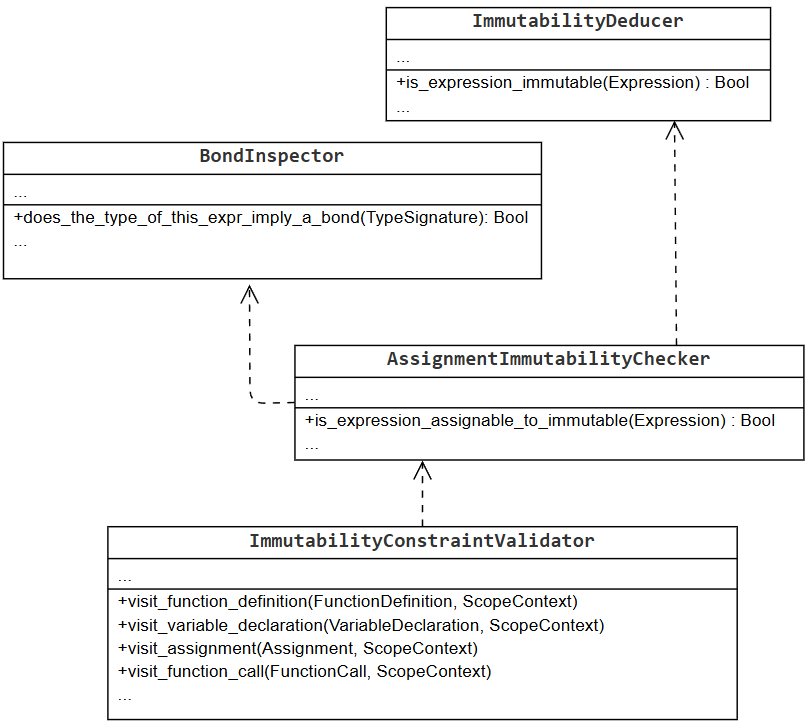
\includegraphics[scale=0.7]{../../Assets/ImmutabilityUML.png}
    \caption{Diagramma UML delle classi che implementano i controlli di immutabilità}
\end{figure}
\vspace{0.5cm}

La classe \texttt{ImmutabilityConstraintValidator} verifica non solo la correttezza degli assegnamenti 
espliciti, ma anche la correttezza degli assegnamenti impliciti, come ad esempio l'assegnamento di un 
argomento di funzione ad un parametro formale e l'assegnamento del valore iniziale di una variabile alla 
suddetta variabile. \\

\newpage

La classe \texttt{ImmutabilityDeducer} è una classe di appoggio con un singolo metodo pubblico. Tale metodo è 
\texttt{is\_expression\_immutable} e serve a navigare l'AST di un'espressione e a restituire \texttt{true} se
tale espressione è immutabile, \texttt{false} altrimenti. La politica applicata nel decretare l'immutabilità
di un'espressione è la seguente:

\begin{itemize}
    \item \textbf{Operatori binari}: sempre immutabili
    \item \textbf{Operatori unari (matematici)}: sempre immutabili
    \item \textbf{Operatori unari (logici)}: sempre immutabili
    \item \textbf{Operatori unari (su puntatori)}: immutabili se è immutabile l'operando
    \item \textbf{Cast}: immutabili se è immutabile l'operando
    \item \textbf{Accessi a membro}: immutabili se è immutabile l'operando
    \item \textbf{Accessi a cella}: immutabili se è immutabile l'operando
    \item \textbf{Chiamate a funzioni}: il valore restituito da una chiamata è \textit{non} immutabile
    \item \textbf{Identificatori}: immutabili se dichiarati come costanti
    \item \textbf{Literali}: sempre immutabili
\end{itemize}

La classe \texttt{AssignmentImmutabilityChecker} verifica se è possibile l'espressione presa in easame 
ad un'espressione destinazione \textit{non} immutabile. Tale classe è utilizzata dalla classe 
\texttt{ImmutabilityConstraintValidator} per ispezionare tutti gli assegnamenti. \\

La politica applicata nel decretare la validità di un assegnamento rispetto all'immutabilità è la seguente:

\begin{itemize}
    \item L'assegnamento è \textit{non-valido} se l'espressione destinazione è immutabile. Per 
    valutare questo criterio ci si affida alla classe \texttt{ImmutabilityDeducer}
    \item L'assegnamento è \textit{non-valido} se l'espressione destinazione è in sola lettura,
    ovvero se mutamenti di tale espressione non sarebbero osservabili in nessun caso. Per valutare
    questo criterio ci si affida alla classe \texttt{OvservabilityDeducer}
    \item L'assegnamento è \textit{non-valido} se esso consentirebbe di modificare indirettamente 
    l'espressione sorgente mediante manipolazione dell'espressione destinazione e l'espressione sorgente 
    è immutabile. Per valutare questo criterio ci si affida alla classe \texttt{BondInspector}
\end{itemize}

Si ricordi che con \textit{espressioni di sola-lettura} si intendono le espressioni che non sono propriamente 
immutabili, ma che qualora mutate non mostrerebbero effetti nel programma di alcun tipo. Un esempio di espressione 
immutabile è una chiamata a funzione che restituisce un non-puntatore (nè vettoriale nè scalare). \\
